\documentclass[pageno]{jpaper}

%replace XXX with the submission number you are given from the ISCA submission site.
<<<<<<< HEAD
\newcommand{\IWreport}{ 2014. Author: David McKenna}
=======
\newcommand{\IWreport}{ 2013. Author: David McKenna, Adviser: Dr. Christiane Fellbaum}
>>>>>>> 5f9a2a1ab9dfe616eeb15c111082ff5489928400
\usepackage{graphicx}

\usepackage[normalem]{ulem}

\begin{document}

\title{
Analyzing Sentiment in the News, and Its Effects on Economic Sectors}

\date{}
\maketitle
\doublespacing
\pagestyle{plain}
\setcounter{page}{1}
\pagenumbering{arabic}

\begin{abstract}
<<<<<<< HEAD
It has been observed that consumer sentiment has a significant impact on the prices of market securities. This paper, based on indendent research done in the Computer Science department, reviews relevant past research literature and investigates which sectors of the economy are most affected by consumer sentiment, by using news articles as a proxy for consumer sentiment. We use ETFs (exchange traded funds), which are basket securities containing many stocks in a given sector, as a measurement proxy for different sectors of the economy. The sectors analyzed are energy, financials, health care, retail, and technology. News articles are categorized by economic sector, and are assigned a numerical score between 0 and 1 based on the sentiment in the article. This continuous classification differs from previous binary classification efforts. These scores are computed by parsing the articles' language, using SentiWordNet to determine word sentiments of adjectives describing keywords and verbs, and weighting words' scores based on their locations in the article. Weights were determined by analyzing movie reviews, which contain scores, with linear regression. One obstacle in parsing language like this is disambiguating word senses. We develop a new approach for disambiguating adjectives using WordNet synsets' sample sentences, and graphical methods based on WordNet synsets to determine the senses of adjectives with their corresponding nouns in our corpus. The results of the analysis suggest tech and retail stocks are most responsive to consumer sentiment, and health care the least.
=======
It has been observed that consumer sentiment has a significant impact on the prices of market securities. This paper investigates which sectors of the economy are most affected by consumer sentiment, by using news articles as a proxy for consumer sentiment. We use ETFs (exchange traded funds), which are basket securities containing many stocks in a given sector, as a measurement proxy for different sectors of the economy. The sectors analyzed are energy, financials, health care, retail, and technology. News articles are categorized by economic sector, and are assigned a numerical score between 0 and 1 based on the sentiment in the article. This continuous classification differs from previous binary classification efforts. These scores are computed by parsing the articles' language, using SentiWordNet to determine word sentiments of adjectives describing keywords and verbs, and weighting words' scores based on their locations in the article. Weights were determined by analyzing movie reviews, which contain scores, with linear regression. One obstacle in parsing language like this is disambiguating word senses. We develop a new approach for disambiguating adjectives using WordNet synsets' sample sentences, and graphical methods based on WordNet synsets to determine the senses of adjectives with their corresponding nouns in our corpus. The results of the analysis suggest tech and retail stocks are most responsive to consumer sentiment, and health care the least.
>>>>>>> 5f9a2a1ab9dfe616eeb15c111082ff5489928400
\end{abstract}

\section{Introduction}

\indent Consumer sentiment has been shown to have a significant influence on the prices of market securities[1][2][3]. While research has shown the correlation between sentiment and market prices broadly, there has been lack of research on the relative effects of sentiment on different industries. It seems intuitively plausible that some industries' prices are more closely determined by facts of nature (oil, gold, etc.) than other industries, the prices of which may be more susceptible to the vagaries of consumer sentiment. This paper aims to discover the effects of sentiment on five different industries: energy, financials, health care, retail, and technology. \\
\indent While there exist myriad sources of data to use as a proxy for consumer sentiment, news articles are particularly well suited for a natural language processing (NLP) based analysis. First they provide a compact and broad reflection of consumer sentiment, as objective journalism typically includes various sentiment viewpoints deemed relevant by the journalist. They are also written in grammatical English, allowing us to use NLP tools like parsing more easily than with a less grammatical corpus like Twitter. Furthermore, they follow a uniform structure, with a title and body, allowing us to use this structure as part of our analysis.
\subsection{Corpus and Overview of Approach}
\indent Our corpus consists of 57 news articles from Bloomberg News, each between about 200 and 1000 words in length. The total length of the corpus is 29,775 words. There are about 10 articles corresponding to each industry. \\
\indent In order to analyze the sentiment of the articles, we maintain a list of keywords for each industry. These keywords are nouns that are especially relevant to each individual industry. Adjectives modifying these nouns correspond approximately to sentiment about the industry. This list of keywords, shown in Table 1, was built by examining the most frequently used words in each set of articles, and using those nouns relevant to the industry. There are 15 keywords for each industry, which happened to be a natural cutoff based on word frequencies. The number of times the word in appeared in the industry's article set appears in parentheses. Note that there is some overlap between industries, with the term "U.S" appearing in  each one. \\
\indent Also note that in building the list, all nouns in the articles were converted to their base forms, using the \textit{inflect.py} Python package. This was done to prevent plural and singular versions of the same noun from being counted separately.

\begin{table}
  \centering
    \begin{tabular}{| l | l | l | l | l | l |}
    \hline
    Energy & Financials & Health Care & Retail & Tech \\ \hline
    energy (45) & U.S. (26) & data (18) & company (21) & company (17) \\ \hline
    U.S. (41) & government (20) & people (16) & sale (20) & telecom (17) \\ \hline
    gas (34) & Shanghai (20) & health (14) & cocoa (16) & stock (14) \\ \hline
    futures (20) & people (16) & air (13) & Chanel (12) & share (12) \\ \hline
    wind (20) & data (15) & fda (13) & growth (11) & Motorola (11) \\ \hline
    oil (20) & KKR (15) & company (12) & Herbalife (10) & Warner (10) \\ \hline
    data (19) & bank (14) & group (12) & Euro (10) & violin (10) \\ \hline
    EIA (15) & office (14) & insurer (11) & China (9) & Italia (10) \\ \hline
    government (14) & holding (14) & cell (11) & car (9) & time (9) \\ \hline
    power (14) & yen (13) & U.S. (9) & people (8) & cable (9) \\ \hline
    prices (13) & group (13) & enrollment (9) & case (8) & internet (9) \\ \hline
    fuel (11) & credit (13) & product (9) & U.S. (8) & U.S. (9) \\ \hline
    inventory (10) & fund (12) & Beijing (8) & price (7) & Microsoft (9) \\ \hline
    Envestra (9) & capital (10) & consumer (6) & ivory (7) & group (8) \\ \hline
    commodity (8) & investor (10) & proposal (6) & auction (6) & market (6) \\
    \hline
  \end{tabular}
  \caption{List of Keywords by Industry}
  \label{table:formatting}
\end{table}

\subsection{Previous Research}
\indent As mentioned earlier, researchers have shown a correlation between consumer sentiment and market security prices. Corredor, Ferrer, and Santamaria showed that investor sentiment had a significant impact on market prices in the UK, Spain, France, and Germany.[1] Baker and Wurgler also showed that investor sentiment has a strong impact on the prices of some securities, most strongly on securities that were difficult to arbitrage or value in general.[2] Baker and Wurgler used an average of six proxies to measure sentiment, including trading volume, dividend premia, and first-day IPO returns, although none of the proxies directly measured sentiment as our approach aims to using NLP. \\
\indent Other related research focused on classifying sentiment by directly analyzing words used in a corpus. Godbole, Srinivasaiah, and Skiena designed a system that assigned a sentiment score to specific entities mentioned in news and blog posts.[5] They created a custom sentiment classification system for WordNet synsets. Similarly to SentiWordNet, it begins with a set of manually classified seed synsets (with polar sentiment), and then classifies all other synsets based on their distance to the seeds. The closer a synset is to a seed, the more weight the seed's sentiment is given in the synset. Like our approach, the researchers assigned continuous rather than binary sentiment scores to entities. Among their findings was that news articles and blogs often had very different sentiments toward notable figures, perhaps pointing to the two media's differing biases. \\
\indent Ohana and Tierney developed a sentiment classification system for film reviews using SentiWordNet.[6] They used adjectives, adverbs, and verbs in the corpus, and the corresponding SentiWordNet values, to evaluate the sentiment of film reviews. Their SentiWordNet-based evaluation predicted review sentiment with accuracy near that of manual classification of words in the corpus, suggesting that SentiWordNet is very powerful in quantifying a word's sentiment. Their approach included only binary classification of corpus documents, and made no effort to disambiguate word senses. In fact, Ohana and Tierney concede that lack of disambiguation contributed to inaccuracy in their approach.
\section{Text Processing and Parsing}
\subsection{Tools and Technologies}
\indent The NLP system used to analyze the sentiment of the news articles was developed in Python, with heavy use of the Natural Language Toolkit (NLTK). NLTK provides libraries for text processing, part of speech tagging, grammar definition, and parsing. \\
\indent The basic operation of our sentiment analysis program works as follows. First, a file containing the relevant corpus is taken as an argument, and it is read into the program line by line. Here, lines correspond to news paragraphs, typically between 1 and 3 sentences. Then the paragraph is parsed into separate sentences using NLTK, and each sentence is tagged by part of speech (i.e. all of its words). Then, the tagged sentence is parsed using the Stanford Parser, which will be discussed shortly, and the resulting parsed sentence is analyzed. The noun phrases for frequently occurring nouns were analyzed by using the SentiWordNet score of the adjective, also discussed shortly, conditional on its disambiguation (discussed in section 4). All verbs tagged are also analyzed using their SentiWordNet score. Finally, the average score per word is computed separately for the article's title and body, and then the weighting algorithm is run to determine the article's sentiment score. \\
\indent These article scores, calibrated using movie review data (discussed in section 3), are then averaged for each industry, and we can compare these scores with the corresponding ETF returns using regression to determine the industries' relation to sentiment. \\
\indent The main tool we use for sentiment classification is SentiWordNet, a "sentiment dictionary" of sorts that assigns a sentiment score to each WordNet sysnet. SentiWordNet and our sentiment scoring system is discussed in detail in section 2.3.
\subsection{Parsing}
As discussed earlier, we want to analyze adjectives and verbs in the corpus to determine sentiment. For verbs, we include each verb we encounter in the sentiment score. But for adjectives, we must determine the noun it is modifying. We need the noun for two reasons: we only include adjectives that modify one of our keyword nouns listed above to keep these sentiment heavy words relevant, and we also use the noun being modified to disambiguate the adjective. \\
\indent Because such "adjective-noun pairs" can occur in a variety forms, we use the Stanford Parser to parse sentences. We first tried to define a limited grammar to capture adjective-noun pairs, but the complexity that these pairs can occur in resists a simple grammar. For example, consider the following sentence: \\
\textit{Consumers who have been affected badly by the recession are anxious to see a turnaround.} \\
If "consumer" is a keyword, then we are interested in the adjective-noun pair "anxious consumers". But defining a limited adjective-noun grammar that is robust to clauses like the one here that separates the noun and adjective is not easy. The Stanford Parser, on the other hand, does a good job parsing sentences like these, and we can quickly look for noun phrases with relevant keywords, and their accompanying modifiers. All adjectives associated with a keyword noun are analyzed for sentiment, in addition to all verbs encountered in a parsing.\\
\indent One other significant detail about our treatment of the parsed sentence is that we always check if a word is preceded by a negating word (like "not"). If this is the case, the sentiment score is multiplied by -1 (to invert the sentiment). In other words, if the sentence above instead read: \\
\textit{Consumers who have been affected badly by the recession are not anxious to see a turnaroud.} \\
then the sentiment score of anxious would be multiplied by -1. \\
\indent The Stanford Parser is a probabilistic parser that uses a learning algorithm to parse a sentence. It uses a class of parsing called \textit{dependency parsing}, which is illustrated in figure 1. For the purposes of our analysis, this parsing structure allows us to track the modifiers of keywords easily, as these modifiers depend on the noun they are modifying. \\
\indent Figure 2 illustrates the dependency parsing of a sentence. Here, if the word "relation" is a keyword, we would include the sentiment score of the word "dependency" in our sentiment analysis. We would also include the word "is" (as we include all verbs).
\begin{figure}
\centering
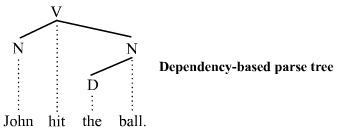
\includegraphics[width=80mm]{Parse.jpg}
\caption{Dependency-based Parse Tree[7]}
\label{overflow}
\end{figure}
\begin{figure}
\centering
\includegraphics[width=90mm]{Parse2.png}
\caption{An example of a parsed sentence[8]}
\label{overflow}
\end{figure}
\subsection{SentiWordNet}
\indent We use SentiWordNet to determine the sentiment of adjectives and verbs. SentiWordNet is a database of sentiment scores for WordNet synsets, assigning scores that range from 0 to 1 in the categories "positive", "negative", and "neutral", and the scores sum to 1 for each synset. An example of a SentiWordNet entry is given in figure 2.\\
\begin{figure}
\centering
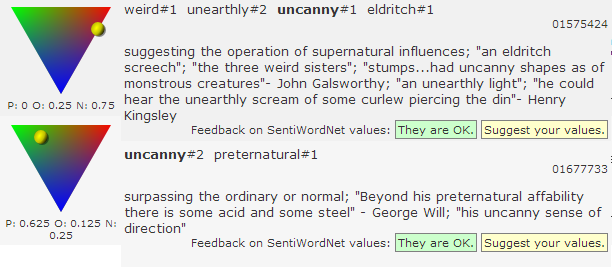
\includegraphics[width=140mm]{sentiwordnet.png}
\caption{SentiWordNet Entry}
\label{overflow}
\end{figure}
\indent SentiWordNet 3.0, the latest version, was used as part of our analysis. This version of SentiWordNet was generated using two small sets of "paradigmatically positive and negative" words. In other words, these sets consist of polar positive and negative words ("good", "bad", etc.). From these manually classified starting sets, binary WordNet relations (synonymy and antonymy) were used to expand the sets. With the expanded sets, and an additional manually classified set of objective words (i.e. words without positive or negative sentiment), all other synsets are assigned sentiment scores using a supervised learning algorithm. The algorithm inspects the definition (or gloss) of each synset, specifically the frequency of each word in the definition, to determine the sentiment score in each of the three categories. After this step finishes, a "random-walk" algorithm is run until convergence. It consists of inspecting the synsets ($s_i$) of words occurring in the gloss of another synset ($s_1$), and changing the sentiment score of $s_1$ based on the sentiment scores of $s_i$. The intuition behind the algorithm is that a synset of with many positive/negative/neutral words in its gloss is probably also positive/negative/neutral.[4] \\
\indent For the purposes of our news sentiment analysis, we need to assign each word a single numerical score based on SentiWordNet's three separate scores. We can easily do this by making a word's sentiment score in our analysis equal to the SentiWordNet positive score minus the SentiWordNet negative score. In figure 2, the first sense of "uncanny" has a sentiment score equal to $0 - .75 = -.75$, and the second sense has a sentiment score $0.625-0.25 = 0.375$. Note that this formula gives a sentiment score in the range $[-1, 1]$.
\section{A Title and Body Weighting Algorithm}
\subsection{Overview and Corpus}
\indent Our approach to sentiment scoring thus far includes inspecting all adjectives and verbs, and using the SentiWordNet positive score minus the negative score. Averaging these sentiment scores gives us some approximation of a news article's sentiment, but it seems easier to convert this arbitrary number to a scoring system we are more familiar with. It also seems intuitively plausible that sentiment laden words in an article's title are more relevant to its general sentiment than words in the body. \\
\indent Movie reviews provide a way to address both of these issues. Movie review writers usually assign a numerical score (stars out of four, for example) that corresponds to their opinion of a film, and reviews usually contain a title and body. As such, we can use a regression based approach, running our analysis on movie review articles separately on title and body, and finding best fit weights, $w_t$ and $w_b$ (for title and body), to multiply our corpus sentiment scores with to obtain sentiment scores for each article. \\
\indent Our corpus consists of 10 movie reviews, linked to on movie review aggregator RottenTomatoes.com. The reviews were chosen for different films, and for a variety of sentiments (i.e. very negative to very positive). \\
\indent Also note that for this corpus, because the reviews were across different movies and genres, we chose not to maintain of list of keywords for adjective inspection. Instead we scored every adjective and verb we encountered.
\subsection{Movie Ratings as Continuous Sentiment Approximation}
\indent Movie reviews provide a stable and familiar basis for continuous sentiment approximation. Consider that if we want to examine a corpus's text to determine a numerical sentiment score, there isn't a much better set of training data than movie reviews. Authors of these reviews assign their own numerical score with the text review, and it seems reasonable that the author is the best judge of the review's sentiment. \\
\indent Of course, using movie reviews as training data also presents some possible problems, which illustrate deeper issues in the field of sentiment analysis. First, it seems that we can't have a perfect mapping between a corpus and sentiment score. Two people who read the same text are unlikely to give it the same sentiment score. Furthermore, it is unclear that two authors would use similar language to express the same sentiment score. A melodramatic author might opt for harsher language. In fact, it isn't clear that authors would share the same sentiment scores about particular senses of a word. \\
\indent Of the movie reviews in our corpus, not all use a uniform ratings system. Some are out of 4 stars and others out of 5 or 10 (but all contain numerical scores of some kind). To standardize these scores, we simple divide the rating given for a movie by the highest possible rating. So 2 stars out of 4 is as good as 5 out of 10 (as both are 0.5 in our input data).
\subsection{Linear Regression for Sentiment Weights}
The basic operation of our movie review regression is as follows. Our movie review articles are separately scored for sentiment, and the title and body of each review is scored for sentiment. This yields a 2x10 matrix ${\bf m}$ of sentiment scores, and we use the Sci-Kit Python package to run a 2 dimensional linear regression with the articles' corresponding reviewer scores. The regression yields the weight constants mentioned earlier, $w_t$ and $w_b$, which are the multipliers for sentiment scores of the title and body of an article. The 2-d linear regression minimizes the squared error of the expression ${\bf w \times m - s}$ where ${\bf s}$ is the 10x1 vector of reviewer scores. \\
\indent The regression determined $w_t = 1.43$ and $w_b = 8.45$ for our data. As a sanity check, it makes sense that both of these numbers are positive (so that the direction of sentiment from our SentiWordNet based analysis agrees with the writer's sentiment score). It also makes sense that the body's score would have more weight than the the title, since the title's score is very levered (i.e. the substitution or inclusion of one sentiment-laden word might very much skew the score). The regression would indicate that a review's title comprises about 15 per cent of its "normalized" sentiment score, with 85 per cent coming from the body of the review.
\subsection{Testing on Out of Sample Data}
To determine if our scoring system with weights is really useful in predicting news article sentiment, we should first determine if it works on out-of-sample movie reviews. We picked 6 reviews from Rotten Tomatoes and ran our with linear regression weights, and the results are listed in Table 2. The first column is the review's title, the second is the critic's assigned score, the third is our system's weighted prediction, the fourth is the (absolute) difference between the two, and the fifth is the absolute error. Absolute error is computed as: \\
\textit{$abs$ $error = \frac{|score-prediction|}{score}$} \\
Also, remember that for an article with title sentiment score $s_t$ and body sentiment score $s_b$, the predicted score $p_s$ is: \\
\textit{$p_s = w_t \times s_t + w_b \times s_b$} \\
\indent The prediction system seems to work reasonably well. If we consider ratings greater than 0.5 positive, and less than 0.5 negative, then the system predicts the polarity of review (binary classification) correctly in 5 of the 6 reviews. The average difference in prediction is .21, and average absolute error is .28. Our admittedly small analysis here suggests the system is reasonable in predicting sentiment scores for movie reviews, and should remain so for evaluating the sentiment of news articles.
\begin{table}
  \centering
    \begin{tabular}{| l | l | l | l | l | l |}
    \hline
    Review Title & Score & Prediction & Difference & Abs Err \\ \hline
    Anchorman 2: The Legend Continues & 0.78 & 1.04 & 0.26 &.333 \\ \hline
    The Hunger Games: Catching Fire & 0.75 & 0.79 & .04 & .053 \\ \hline
    DiCaprio and Scorsese..."The Wolf of Wall Street" & 0.625 & 0.72 & .095 & .152 \\ \hline
    The Diva Review: "The Wolf of Wall Street" & 0.5 & 0.59 & .09 & .18 \\ \hline
    'Saving Mr. Banks': A Spoonful of Sugar Helps... & 0.75 & 0.31 & .44 & .59 \\ \hline
    ‘Philomena’: Judi Dench shines in this ... drama & 0.875 & 0.99 & .115 & .116 \\ 
    \hline
  \end{tabular}
  \caption{Out of Sample Film Review Test Data}
  \label{table:formatting}
\end{table}

\section{Disambiguation}
\subsection{State of the Art of Disambiguation}
Disambiguation is an open problem in NLP. It refers to finding the right dictionary sense of a word used in a corpus. For example, figure 3 shows two separate senses of the word "uncanny". So while \textit{an uncanny specter} uses the first sense of the word, \textit{her uncanny ability} uses the second sense. In terms of our sentiment analysis, note that the two senses have opposite sentiment polarities (-.75 vs. +.375). \\
\indent A variety of algorithms have been used for disambiguation. Lesk's algorithm was introduced by Michael Lesk in 1986. The simplified version of the algorithm disambiguates a corpus word ${\bf w}$ by inspecting the definition of each sense of ${\bf w}$ and also any sample sentences, and chooses the sense that contains the most overlap with the sentence in the corpus where ${\bf w}$ is used. Overlap is taken to mean the number of words in common.[9] One immediate problem with the simplified version of Lesk's algorithm is that it is very sensitive to the particular words used in the definition. In particular, if ${\bf w}$ is "uncanny", and the corpus sentence also contains the word "eerie", there will be no overlap with either gloss. This will happen despite the first gloss containing synonyms and related words like "supernatural", "weird", and "unearthly". \\
\indent Supervised and semi-supervised machine learning algorithms have been used extensively.  Among these algorithms is the Yarowsky algorithm. This semi-supervised learning algorithm disambiguates based on collocations, or word pairings, in the labeled text. This approach is effective in disambiguating phrases like "play bass" versus "play ball".[10] One issue with learning techniques is that they are sensitive to labeled input data. If the style of either the labeled data or the test data varies greatly from the other, the learning algorithm might be less effective. \\
\indent There are some serious theoretical problems associated with disambiguation that make it a particularly hard problem. First, dictionaries often contain varying entries of the same word. Consider that the American Heritage Dictionary has only one entry for the word "uncanny" that combines the senses listed in WordNet (it defines uncanny as "mysterious or impossible to explain especially when causing uneasiness or astonishment").[11] It seems that if two dictioary editors cannot agree on the different senses of a word that can be defined, then we won't be able to disambiguate the word effectively in a corpus. A related problem is that humans often disagree on which sense of a word is being used in a corpus.[12]
\subsection{WordNet Based Approach for Disambiguating Adjectives}
\indent We implement a new algorithm for disambiguating adjectives in our sentiment analysis. Our technique for disambiguation attempts to overcome the narrow gloss sensitivity of Lesk and the stylistic sensitivity of learning algorithms by relying on WordNet sample sentences and relationships. \\
\indent First note that we maintain adjective-noun pairs in our corpus, so that we have the corresponding noun that each adjective is modifying. Also note that WordNet typically contains sample sentences for each adjective synset (i.e. each different sense of adjective). By parsing these sample sentences, we can determine the nouns that are being modified. The intuition behind our approach is to try to connect the noun being modified in the corpus to the noun(s) being modified in the synset's sample sentence(s). \\ \indent Note that the only nouns we inspect in our corpus are the keywords listed in table 1. If the noun is not in WordNet (i.e. company names like Microsoft), we do not attempt to disambiguate its modifier, so we just use the first sense listed in these cases. \\ 
\indent Our algorithm maps each keyword to its "branch" up the WordNet tree all the way to "entity" (the root of these WordNet nouns). As an example, here is the branch of the keyword government: \\
\textit{government $\Rightarrow$ organization $\Rightarrow$ social group $\Rightarrow$ group $\Rightarrow$ abstraction $\Rightarrow$ entity} \\
Here "organization" through to "entity" are \textit{hypernyms} of the "government" synset, satisfying the "is-a" relationship. \\
\indent When we encounter an adjective-noun pair ${\bf \{a,n\}}$ in the corpus that we want to disambiguate, we find the branch of ${\bf n}$ that we built (${\bf b_n}$). Then we inspect the WordNet sample sentences for the synsets (senses) of ${\bf a}$, and specifically the nouns being modified. Their set of branches corresponding to these nouns ${\bf \{b_a\}}$ are also stored. For each of these branches, we seek the branch with the deepest common overlapping hypernym. In other words, for an adjective with two synsets, if the the branch of the first noun overlaps at "group" (and hence at "abstraction" and "entity" also), and the second overlaps at "organization" (and hence at "social group", etc.), we would pick the adjective second sense. If branches are tied for the deepest overlapping hypernym, we instead look for the noun sense that maximizes the path similarity score. Path similarity is a measure of the shortest hypernym path between two words. Path similarity is a function built into the WordNet extension of the Natural Language Tool Kit.
\subsection{An Example}
To illustrate our algorithm's operation, consider the following sentence we find in a corpus: \\
\textit{For the first time in centuries, the country is reaping the benefits of democratic government.} \\
\indent Here, we want to disambiguate the adjective "democratic" modifying the keyword "government". We find the two WordNet synsets corresponding to the word "democratic". The first, defined as "characterized by or advocating or based upon the principles of democracy or social equality", contains the sample phrase: \textit{a democratic country}. The second is defined as "representing or appealing to or adapted for the benefit of the people at large", and contains the sample phrase: \textit{democratic art}. Next, we trace the hypernym branches of "country" and "art": \\
\textit{country $\Rightarrow$ political unit $\Rightarrow$ unit organization
 $\Rightarrow$ social group $\Rightarrow$ group $\Rightarrow$ abstraction $\Rightarrow$ entity} \\
\textit{art $\Rightarrow$ creation $\Rightarrow$ artifact $\Rightarrow$ whole $\Rightarrow$ object $\Rightarrow$
physical entity $\Rightarrow$ entity} \\
We find that the deepest common overlapping hypernym for "country" with "government" is "social group", and that the deepest for "art" is "entity". The depth of "social group" is 3, and the depth of "entity" is 0, so we choose the first sense of "democratic". Indeed, it seems that this is the reasonable choice for the phrase "democratic government".
\section{Results of Analysis}
\begin{figure}
\centering
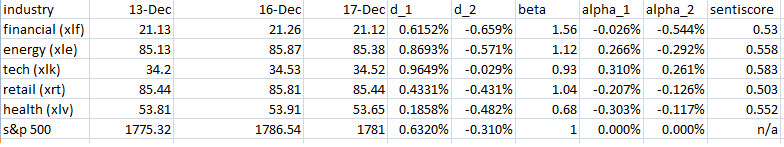
\includegraphics[width=167mm]{sentiscores.png}
\caption{Results of Sentiment Analysis}
\label{overflow}
\end{figure}
Figure 4 shows the results of applying our sentiment scoring system to the corpus of industry news articles. We first discuss the financial aspects of the evaluation, and then discuss the accuracy and significance of the results.\\
\indent The ETFs chosen to proxy the five industries were the Standard and Poor's funds corresponding to each industry (also called SPDR funds). Recall that ETFs are basket securities containing many stocks of a single sector, and thus provide a picture of what is happening in the sector as a whole. While many different ETFs are available to act as a proxy for each industry, choosing the corresponding SPDR funds gives us a consistent and less arbitrary basis than choosing a grab bag of different ETFs for each industry. The first column in the results table lists the industry and ticker symbol of its corresponding SPDR ETF.\\
\indent The trading days listed are the trading day before the publication of the articles (12/13), the trading day of their publication (12/16), and the trading day after publication (12/17). The second, third, and fourth columns list the prices of the respective securities on these days. The fifth column ($d_1$) is the percent change in the security price from 12/13 to 12/16, and the sixth column ($d_2$) is the percent change in the security price from 12/16 to 12/17. \\
\indent Next, we come to the issue of quantifying the sector specific changes in securities. At a high level, all securities are correlated to some degree with the general return of the market, here proxied by the S and P 500 index. In order to examine sector specific changes in prices, we need to account for this correlation. Luckily, the Capital Asset Pricing Model (CAPM) allows us to do this easily enough. The CAPM model says that an asset's expected return $r_a$ can be related to the market return $r_m$, the asset's beta coefficient with the market (basically its correlation with market returns), the risk free borrowing rate $r_f$, and any other "abnormal" or security specific fluctuation $\alpha$. The formula can be stated as $r_a = r_f + \beta (r_m - r_f) + \alpha$. For our purposes, we would like to know how sentiment affects the unusual return of the ETF, captured in its $\alpha$. In other words, the $\alpha$ term should capture whatever to a sector happens independently of what would be expected based only on other stocks. So the seventh column is each security's beta coefficient, and columns eight and nine indicate the alpha return from December 13th to 16th, and 16th to 17th respectively. Note that because risk free borrowing rates were negligible on these dates relative to the market return rate, we have neglected $r_f$ here. Finally, the tenth column lists the sector's sentiment score, using our analysis. This is the average sentiment score of each set of articles for each sector. So if the sentiment score is 0.5, this would mean an average sentiment of 2 out of 4 stars per article for the industry (in movie review lingo).\\
\indent To analyze our results more rigorously, we perform a linear regression between sentiment score and alpha return for the two days. Figure 5 displays the regression between sentiment and alpha for the returns on 12/16, and figure 6 shows the regression for the returns on 12/17. \\
\begin{figure}
\centering
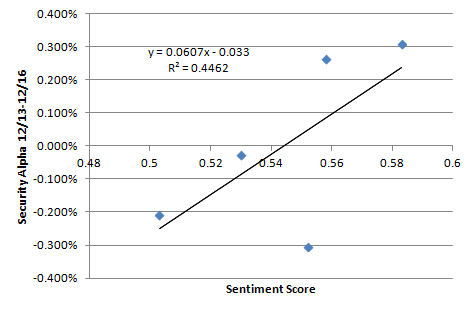
\includegraphics[width=115mm]{returns1.png}
\caption{Sentiment-Alpha Regression for 12/16}
\label{overflow}
\end{figure}
\begin{figure}
\centering
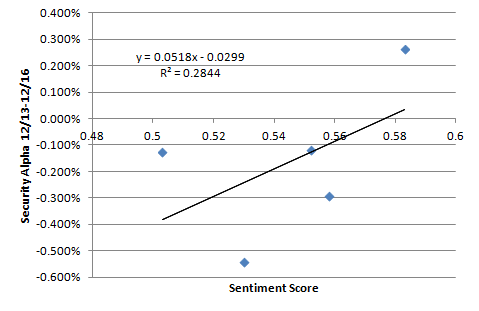
\includegraphics[width=115mm]{returns2.png}
\caption{Sentiment-Alpha Regression for 12/17}
\label{overflow}
\end{figure}
\indent Qualitatively, the regression graphs both show a positive trendline from sentiment score to alpha. This is what we would expect if sentiment does indeed correlate with market returns. Both sets have significant outliers, demonstrating that the system isn't perfectly effective. The first graph, which measures alpha returns for 12/16, captures the relationship between news sentiment, and returns on the day the news was written. Almost all of the articles in the corpus were published after the market's closing, so this graph can be interpreted as "reactive sentiment," so causality would point from market events to sentiment. The second graph, with alpha returns for 12/17, effectively measures the market's reaction to sentiment, so causality would point from sentiment to market activity ("predictive sentiment"). \\
\indent Quantitatively, the coefficient of determination ($R^2$, displayed on the graphs) for the 12/16 data is 0.4462, and for 12/17 is 0.2844. This suggests the trendline is more accurate for the 12/16 data, and would point to "reactive sentiment" as the correct interpretation of the market's behavior regarding consumer sentiment. \\
\indent Another quantitative observation we can make is that tech and retail stocks are the best predicted sectors by our consumer sentiment regression, and health care stocks the worst. The former two have the least residual squares summed over the two days (5.86e-6and 6.84-6 respectively), and health care has the highest (1.255e-5). This also seems to agree with qualitative observation of sentiment and alpha return on the graph, assuming a positive correlation exists. A rough economic interpretation for this may be that tech and retail stocks depend more on the vagaries of consumers feelings than a sector like health care, which may be more responsive to political happenings.
\section{Evaluation of Research}
Our research suggests that there is indeed a correlation between consumer sentiment and market prices, but one that is probably more reactive than predictive. It also suggests that not all industries are affected equally by sentiment, with tech and retail more responsive to sentiment and health care less so. \\
\indent We could improve our understanding of the link between sentiment and industry prices by considering more industries, using a larger corpus of news articles, and investigating the link over a longer period of time. We might also use a different sentiment scoring system to see if the results are sensitive to this choice, and a different corpus, like Twitter, for similar reasons. \\
\indent Our methodology used SentiWordNet to analyze the corpus's sentiment, and also utilized a new method to disambiguate adjective senses. Based on the results of our movie review tests and market data, it seems to have been an effective approach in analyzing sentiment. \\
\indent There is room for improvement in our methodology, also. The disambiguation algorithm could be extended to include verbs and other parts of speech. Another way to improve the disambiguation algorithm would be to use a larger corpus, and cluster similar senses of adjectives first, and then compare them to WordNet sample sentences.\\
\\
{\bf References} \\
1. Corredor, Pilar and Ferrer, Elena and Santamaria, Rafael, Investor Sentiment Effect in 
Stock Markets: Stock Characteristics or Country-Specific Factors? (September 30, 2011). \\
2. Baker, Malcolm, and Jeffrey Wurgler. 2007. "Investor Sentiment in the Stock Market." 
Journal of Economic Perspectives, 21(2): 129-152. \\
3. Cliff, Michael T. and Brown, Gregory W., Investor Sentiment and Asset Valuation (November 19, 2001). \\
4. Baccianella, Stefano, and Esuli, Andrea, and Sebastiani, Fabrizio, SentiWordNet 3.0: An Enhanced Lexical Resource
for Sentiment Analysis and Opinion Mining. \\
5. Godbole, Namrata, and Srinivasaiah, Manjunath, and Skiena, Steven, Large-Scale Sentiment Analysis for News and Blogs (2007).\\
6. Ohana, Bruno and Tierney, Brendon, Sentiment Classification of Reviews Using SentiWordNet (October 1, 2009). \\
7. "Parse tree DG." \textit{Wikipedia}, December 21, 2011. Web. December 4, 2013. http://en.wikipedia.org/wiki/File:Parse2.jpg. \\
8. "tree illustrating the dependency and constituency relations." \textit{Wikipedia}, November 29, 2011. Web. December 4, 2013. http://en.wikipedia.org/wiki/File:Thistreeisillustratingtherelation(PSG).png. \\
9. Michael Lesk. 1986. Automatic sense disambiguation using machine readable dictionaries: how to tell a pine cone from an ice cream cone. In Proceedings of the 5th annual international conference on Systems documentation (SIGDOC '86), Virginia DeBuys (Ed.). ACM, New York, NY, USA, 24-26. DOI=10.1145/318723.318728 http://doi.acm.org/10.1145/318723.318728 \\
10. Yarowsky, D. "Unsupervised Word Sense Disambiguation Rivaling Supervised Methods". 
Proceedings of the 33rd Annual Meeting of the Association for Computational Linguistics. 
Cambridge, MA, pp. 189–196, 1995. \\
11. "uncanny." \textit{The American Heritage Dictionary}, 2013. Web. Decemeber 12, 2013. \\
12. Snyder, Benjamin, and Martha Palmer. "The English all-words task." Proceedings of 
Senseval-3: The Third International Workshop on the Evaluation of Systems for the Semantic 
Analysis of Text, ACL2004. July 21-26, 2004, Barcelona, Spain: 2004  \\
\end{document}

